%%%
%% File       : UserGuide.tex  
%% Maintainer : All 
%% Info: 
%%    See also: vlDefs.tex for the used tyles and aliases.  
%%  

%% TODO: 
%%
%% - UserGuide style document 
%% - Update labels and references
%%  

%% Start of document
\documentclass [a4paper,10pt,twoside]{report}

%% packages 
\usepackage{graphicx}
\usepackage[english]{babel} 
%%% Not Used Packages/Missing packages !!!
\usepackage{fullpage}
%%\usepackage{fancyhdr}
%%\usepackage{fancyvrb}
%%\usepackage{letterspacing}
%%\usepackage{listings}
\usepackage{color}
\usepackage{alltt}
\usepackage{boxedminipage}

%% usefull for reviewing:
%\usepackage[pagewise]{lineno}

%% Following line most be specified as LAST package:
%% enable hyperlinks in PDF file: 
\usepackage[colorlinks=true, pdfstartview=FitV, linkcolor=blue, 
            citecolor=blue, urlcolor=blue]{hyperref}
%%
%% The VLeT style commands: 
%%
%% You are encouraged to add own styles and aliases to this file 
%% Especially acronyms and other common used terms like 'Linux' 
%% VLET_INSTALL, etc 
%%

% personal formatting commands: 

\newcommand\Mail[1]{\texttt{#1}}
%%\newcommand\Url[1]{\texttt{#1}}
\newcommand\Script[1]{\texttt{#1}}
%% URL text format, NOT A HYPERLINK
\newcommand\Text{\textnormal}
\newcommand\Bold[1]{\textbf{#1}}
\newcommand\Variable[1]{\textsf{#1}}
\newcommand\Menu[1]{\textsf{#1}}
\newcommand\Path[1]{\textbf{\texttt{#1}}}
\newcommand\File[1]{\Path{#1}}
\newcommand\Note[1]{\textbf{\underline{#1}}}
\newcommand\Emph[1]{\textit{#1}}
\newcommand\EmphBold[1]{\textit{\Bold{#1}}}
\newcommand\Class[1]{\texttt{#1}}
\newcommand\Code[1]{\texttt{#1}}
\newcommand\Link[1]{\texttt{#1}}
% references: 

%% aliases to ensure consistent usage of name/file/terms etc : 
%% terms/concepts/names 

\newcommand\linux[0]{\textbf{Linux}}
\newcommand\Linux[0]{\textbf{Linux}}
\newcommand\globus[0]{\textbf{GLOBUS}}
\newcommand\windows[0]{\textbf{Windows}}
\newcommand\vletrc{\Path{vletrc}}
\newcommand\myvle{\texttt{MyVLe}}
\newcommand\LocalSys{\texttt{Local System}}
\newcommand\GridHood{\texttt{Grid Neighbourhood}}
\newcommand\VOGroup{\texttt{VO Group}}
\newcommand\VO{\texttt{VO}}
\newcommand\vlet{\texttt{VLET}}
\newcommand\link{\texttt{Link}}
\newcommand\vbrowser{\texttt{VBrowser}}
\newcommand\rightclick{\Bold{right-click}}
\newcommand\python{\texttt{Python }}
\newcommand\dutchgrid{\texttt{DUTCHGRID}}

% some recurrent environment variables 
\newcommand\VLETINSTALL{\Variable{VLET{\_}INSTALL}} 
\newcommand\VLETCONF{\VLETINSTALL/etc/vletrc.prop}
\newcommand\VLETUSERCONF{\HOME/.vletrc/vletrc.prop}
\newcommand\HOME{\Variable{HOME}} 
\newcommand\VLET{\Variable{VLET}}
 
% \newcommand\cpp{\texttt{C++}}

%% misc: 
% couldn't find a windows 'backslash' command so the mathematical \backslash is used: 
\newcommand\bsl[0]{$\backslash$}
\newcommand\rarr[0]{$\rightarrow$}
\newcommand\larr[0]{$\leftarrow$}
\newcommand\lt[0]{$<$}
\newcommand\gt[0]{$>$}

% same for simple 4 character wide TAB (Should be outlined with some indentation)
\newcommand\tab{\hspace*{4ex}} 
\newcommand\step{\hspace*{4ex}\textbf{-}\ } 

%%
%% simple listing commands: 
\def\boxedlisting{ \hspace*{10mm}\begin{boxedminipage}{150mm}}
\def\endboxedlisting{\end{boxedminipage}\\}

 

%\lstloadlanguages{C++,Java}
%% 
%% Begin of document 
%%
\begin{document} 

%% Enable linenumbers for reviewing. Also uncomment %\usepackage{lineno}
%\linenumbers

%% Frontpage
%
% Frontpage for the VLeT UserGuide
% 

\begin{center}
\begin{figure}[htbp]
\centerline{\includegraphics[width=18.00cm]{vle_logo}}
\end{figure}

\vspace{2cm} 

{\Large Virtual Laboratory for e-Science}\\
{\Large The VL-e Toolkit}\\ 

\vspace{1cm} 
 
{\Huge The VL-e Toolkit Installation and User\'{}s Guide}\\ 

\vspace{1cm} 

{(For version 1.5)}\\
\vspace{0.5cm} 
%% TODO: MORE information 
\vspace{0.5cm} 

\Mail{vlet-develop (at) lists.sourceforge.net}\\
\Mail{http://www.vl-e.nl/vbrowser}\\
\end{center}

 
\newpage

%% Colofon  
% COLOFON 

% local style definitions 

\setlength{\parindent}{0pt}
\setlength{\parskip}{1em}

%%TODO: more/better information 

\vspace{10cm} 
\textbf{Netherlands eScienceCenter} \\
Science Park 140 (Matrix I)\\
1098 XG Amsterdam\\
The Netherlands \\
\\
\Bold{Information:} \\
Mail: \Mail{vlet-develop (at) lists.sourceforge.net} \\
Web: \Path{http://sourceforge.net/projects/vlet/} \\
 
\newpage

%% Table of Contents  
\tableofcontents
\newpage
\newpage 

%% My Style Settings (After Table of Contents!) 
\setlength{\parindent}{0pt}
\setlength{\parskip}{1em}
%%\lstset{language=C}
\newcommand{\cpp}{\texttt{C++ }}

%% Chapter 1 
\chapter{Introduction}
\label{sec:Introduction}
\Bold{The VL-e Toolkit.}


%% Add Abstract ? 


This is the Installation and User Guide to the VL-e Toolkit (\vlet) and its
main front-end the \vbrowser. 
This document introduces you to the vlet and vbrowser 
environment and is divided into the following parts: 

\begin{itemize} 
  \item 
    Part I: Introduction \& Installation: Chapter 1 and 2.
  \item 
    Part II: Using the VL-e Toolkit: Chapter 3 and 4. 
  \item
    Part III: Advanced features and customizing settings: Chapter 5.  
  \item
    Appendices.  
\end{itemize} 

Please report any problems, bugs to: \Mail{vlet-develop (at) lists.sourceforge.net} with the subject: 
'\Mail{bug report}' (This is a moderated list, so you may receive a
notification that your message is pending 'approval'). \\
For more information see the site at \Mail{http://www.vl-e.nl/vbrowser} or the
sourceforge project site: \Mail{http://sourceforge.net/projects/vlet/}.


 
\newpage


%% Chapter 2 
%
% Installation
%

%%%%%%%%%%%%%%%%%%%%%%%%%%%%%%%%%%%%%%%%%%%%%%%%%%%%%%%%%%%%%%%%%%%%%%%%%%%%%%%
%                  <--- 80 characters width --> 		                      %
%%%%%%%%%%%%%%%%%%%%%%%%%%%%%%%%%%%%%%%%%%%%%%%%%%%%%%%%%%%%%%%%%%%%%%%%%%%%%%%

\chapter{Installation}
\label{chap:vlet_installation}

\section{Installation requirements}

The VL-e Toolkit has the minimal following installation requirements:
\begin{itemize}  
   \item SUN Java 1.6 JRE (Java Runtime Environment) or JDK is recommended.   
   \item Either Windows 2000/XP/7 or a recent Linux distribution (2.6 kernel)
   \item Other Java 1.6 capable platforms might work as well, but not all
   architectures have been tested. (Mac Os has been reported to work as well).\\
   Alternative Java implementations like 'gcj'  and 'openjdk' might not fully
   support Swing applications which is mandatory for the VBrowser. 
 \end{itemize} 

Also, to be able to access grid resources, you MUST have a grid certificate. 
For instructions how to get one, see:
\url{http://certificate.nikhef.nl/request} or ask your local grid administrator. 

\section{Unpacking}

 Unzip the package with winzip (windows) or gunzip (linux). 
 The installation directory into which you installed it, will be referred to
 as \VLETINSTALL. \\
 \\
 Default installation path on Linux (system wide) installation could be: \\
 \\
 \tab \path{/opt/vlet}\\
 \\
 The installation path on Linux for non system administrators, could be:\\ 
 \\
 \tab \path{\$HOME/vlet}\\
 \\%%$
 Default installation path for a windows (system wide) installation
 could be: \\
 \\
 \tab \path{C:\vlet}\\ 
 \\	
 As users do not need write access to the installation path nor administrator
 rights to install or run parts of the VL-e Toolkit, any user can install it 
 at the desired place he or she wants to.\\
 After unpacking the VL-e toolkit can be used directly by starting the desired
 application or tool from the \path{VLET_INSTALL/bin} directory. Most users don't have 
 to configure their installation and should be able to use the tools right out
 of the box.
 For custom configurations, see the next chapters for an explanation of
 optional properties and installation settings.\\
 
 \subsection{Quick Installation Steps}
 Quick install steps for the impatient are as follows:
 
 \begin{itemize} 
   \item Unzip the vlet distribution. 
   \item Put your personal grid certificate (userkey.pem and usercert.pem) in
         your \HOME/.globus directory. Create the \path{.globus} directory if
         it doesn't exists yet. 
   \item Optionally create a shortcut to \path{VLET_INSTALL/bin/vbrowser.exe}
         (for \windows) and copy the shortcut to your desktop.
   \item Start \path{vbrowser.sh} or \path{browser.exe} from
          \path{VLET_INSTALL/bin} (or use shortcut). 
   \item Optionally, the \path{vbrowser.jar} can be used to directly start the
          vbrowser using any Java Environment (for Mac OS this is the only
          supported way) as follows: \path{java} \path{-jar} \path{vbrowser.jar}
   \item Configure firewall settings by right-clicking (alt mouse button) on the 
         \myvle\ icon seen in Figure \ref{fig:myvle_icon}, select \Menu{properties} and set \Menu{passiveMode} to
   \Menu{true} for firewalled users, or specify an incoming port range if you
         allow incoming tcp/ip connections.
	  
	  \begin{figure}[htbp]
	    \centerline{
\includegraphics[scale=1.0]{vle-world}}
	    \caption{The \myvle\ Icon}
	    \label{fig:myvle_icon}
	  \end{figure}

   \item Optionally put extra CA certificates in your  
         \path{HOME/.vletrc/certificates} directory if CA certificates can't be
         found. This is necessary for non-\dutchgrid\ sites. 
 \end{itemize} 
 
\subsection{Directory structure}

Below an overview of the directory structure of the installation. Only relevant
files and directories are listed here. 

\begin{boxedlisting}
\begin{verbatim}
# Directory structure of VLET distribution: 

ReleaseNotes.txt        # latest release notes.
README.txt              # general README.
INSTALL.txt             # extra installation notes. 
ReleaseNotes.txt        # latest release notes.
LICENCE.txt             # Apache Licence 2.0.
bin/                    # scripts and (binary) executables.
bin/vbrowser.sh         # UNIX (Linux) VBrowser startup script. 
bin/vbrowser.exe        # Windows VBrowser startup executable.
bin/vbrowser.jar        # Java executable jar file.
etc/                    # configuration files. 
etc/vletrc.prop         # installation settings.  
etc/vletenv.sh          # extra Unix/Linux environment settings. 
etc/certificates/       # root CA certificates needed for authentication of 
                          remote hosts.
doc/                    # documentation and Java API (javadoc) files. 
lib/                    # libraries and needed jar files including icons.
lib/plugins             # custom viewers and plugins both for VDrivers and 
                          Viewer Plugins.  
lib/icons               # custom icons. 
lib/icons/mimetypes     # custom mimetype icons.
py/                     # Java Python (Jython) examples.  
\end{verbatim}
\end{boxedlisting}


\subsection{Configuring vbrowser.ini for Windows}

Under Windows, the file 'vbrowser.exe' (located in the 'bin' directory) starts
the VBrowser.
This executable uses the default Java version installed and starts the Java
executable jar file 'vbrowser.jar'. 
If you want to specify an alternative java installation, or the default java
installation can't be found, you can specify it in a configuration file
'vbrowser.ini' located in the same directory as 'vbrowser.exe'.
\\
If on windows VLET is installed in for example \Path{C:\bsl vlet\bsl } you can
create the file \Path{vbrowser.ini} at the following path:\\

	\tab \Path{C:\bsl vlet\bsl bin\bsl vbrowser.ini} 

In that file you can add the following lines:

	\tab \Path{\#\#}\\
	\tab \Path{\# Use following Java installation:}\\
	\tab \Path{java.home=C:\bsl Program Files\bsl Java\bsl jdk1.7}\\

You don't have to put the path between quotes, but make sure no extra spaces are
after the last part of the path (\Path{..\bsl jdk1.7}).\\
Also you can specify extra Java VM options, for example to increase the Java
memory settings: 

	\tab \Path{\# Extra Java VM options. Increase heap size:}\\
	\tab \Path{java.vmargs=-Xms256m -Xmx512m}
	
	
\subsection{Configuring the installation}

 The next sections explains how to configure the default settings in your
 installation. 
 Most settings can be changed interactively through the \vbrowser\ as well.
 You can do this by right-clicking (or use alt-mouse button) on
 the \myvle\ icon or specified resource.
\par
 See the file \VLETCONF\ for (advanced) installation configuration. All the
 variables can also be specified for each user in the
 \path{HOME/.vletrc/vletrc.prop} which overrides default installation settings. (see
 Section: \ref{sec:user_configuration}). As this file changes per distribution,
 see the comments before each property and which are the optimal defaults for your
 distribution and your environment. \\


\section{Configuring Grid Certificates}


\subsection{Configuring your personal Grid certificate}
\label{sec:user_configuration}

The next paragraphs explain where you can find/store your grid certificate
depending on the operating system you are using. 

\subsubsection{Grid certificate directory for \Linux}

 The default location to store your grid certificate for \Linux\ is:
 
 	\tab \path{HOME/.globus}  

 This is the location where the Globus Commodity Grid Toolkit (CoG) stores its
 configuration files. This location is the recommended place for Linux and
 windows users to store their grid certificates (See next section how to find
 your windows home).
 
\subsubsection{Grid certificate directory for \windows}
 
 The default location for \windows\ (XP) could be (depending on the default
 user's home): 
 
	 \tab \Path{C:\bsl WINDOWS\bsl profiles\bsl (Your User Name)\bsl .globus}

 Or on Windows 7, this could be: 
 
 	 \tab \Path{C:\bsl Users\bsl (Your User Name)\bsl .globus}
 	
 The \Path{C:\bsl WINDOWS} part is the prefix where windows is installed. 
 The \Path{.globus} is the directory where the Globus Commodity Grid
 Toolkit (CoG) stores its  configuration files. \\
 If you don't know how to find your Windows \HOME\ you can also just start the
 \vbrowser\ and your home path will be the first resource under the \LocalSys\ icon. 
 This home resource is recognizable by the folder icon
 which has a little house in it as you can see in Figure \ref{fig:home_folder_in_tree}.
 
  \begin{figure}[htbp]
  \centerline{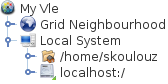
\includegraphics[scale=1.0]{home_folder_tree}}
  \caption{Your HOME folder under window and Linux}
  \label{fig:home_folder_in_tree}
 \end{figure}
 
 Alternatively you could store your certificates into
 another location, or keep a copy, for example the following location:
 
 	 \tab \Path{C:\bsl My Documents\bsl globus}
 
 When installing your grid certificates into another location than the default, 
 you need to configure the VBrowser to search for this location. 
 This will be explained in Section \ref{sec:grid_proxy_configuration}. 
 
\subsubsection{Your Grid Certificate files}

 The files which must be present in your globus certificate directory
 (\path{HOME/.globus}) are:

 \begin{itemize} 
   \item \File{userkey.pem} : 
     Your \Emph{private} grid certificate. Never share this file with anyone. If you 
     loose this file, you'll need to reapply for a new grid certificate. 
   \item \File{usercert.pem} : 
     Your \Emph{public} grid certificate. This file is send over the internet to 
     identify you as the person defined in your grid certificate. Together
     with the \File{userkey.pem} it forms your \Emph{public-private} keypair. 
  \end{itemize} 
  
 For more about \Emph{public-private} keypair encryption, see: \cite{PKCS}.
 
 Optionally this directory may contain the following files: 

 \begin{itemize} 
   \item \File{cog.properties} : 
     This file contains the Globus Commodity Grid (CoG) Toolkit properties.
 \end{itemize} 
 
 \Note{Note}: The \File{cog.properties} file is \Emph{always} stored in the default
 globus configuration directory (\Path{.globus}) in your \HOME\ directory. If this 
 file is present it will override any configurations made in \VLETCONF\ or 
 \path{HOME/.vletrc/vletrc.prop}

\subsection{Configuring host or ``root CA'' certificates} 

The default place to store host certificates under \Linux\ is:\\

	\tab \Path{/etc/grid-security/certificates}\\
	
If you don't have the rights to add/install certificates to this place, you can 
add new certificates to the following location: 

	\tab \VLETINSTALL\path{/etc/certificates}

Or to add root CA certificates to your user environment put them in: 

	\tab \path{HOME/.vletrc/certificates} 

Certificates added to the above locations are loaded automatically
when starting tools from the VL-e toolkit. 
For windows users replace the \path{HOME} variable with your user profile
location. 

For access to \dutchgrid\ sites, no extra configuration should be necessary. To
access other (non \dutchgrid) sites, add your root CA certificate to one of
the above custom locations. 

More information about Grid Certificates can be found here: \cite{288111}


\subsection{Advanced certificate configuration settings}
See the installation file \path{VLET_INSTALL/etc/vletrc.prop} or the user
configuration file \path{HOME/.vletrc/vletrc.prop} for advanced
grid configuration settings. 
Explanation of these properties can be found in Section:\ref{sec:properties})

%%%
%%% Section 
%%%

\section{Properties and configuration settings}
\label{sec:properties}

In the next (sub)sections an overview of the most important settings which can
be specified either installation wide in the \VLETCONF\ file or in the user's
configuration file \VLETUSERCONF. 


%%% --------Obsolete-------------------
% \subsection{Configuring default Resource settings} 
% 
%  The installation file \path{VLET_INSTALL/etc/vletrc.prop} also contains default
%  resource settings for SRB and LFC. When creating a new Resource Location, the default 
%  settings from this file will be used. This file contains \Emph{installation} wide 
%  settings and  may not contain user specific configuration details.\\
%  The location of this file is: 
% 
% 	\tab \path{VLET_INSTALL/etc/vletrc.prop}
% 	
% For example, the default SRB configuration to access the SRB server at SARA is: 
% 
% \begin{boxedlisting}
% \begin{verbatim}
% ##
% # File    : vletrc.prop 
% # Location: $VLET_INSTALL/etc/vletrc.prop 
% # ---
% 
% # ...  
% 
% # Default SRB settings file for SRB server at SARA 
% 
% # Default SRB host at SARA :
% srb.hostname=srb.grid.sara.nl
% srb.path=/VLENL/home
% srb.port=50000
% srb.mdasCollectionHome=/VLENL/home
% srb.mdasDomainHome=vlenl
% srb.mdasDomainName=vlenl
% srb.defaultResource=vleGridStore
% #srb.username=
% srb.mcatZone=VLENL
% # set to true when behind a firewall (Default)
% # if incoming connection are allowed set to 'false'
% srb.passiveMode=true
% #this string MUST match the Enum Value for 'GSI_AUTH'
% srb.AUTH_SCHEME=GSI_AUTH
% 
% # end srbsettings.prop file 
% \end{verbatim}
% \end{boxedlisting}  
%  
% \Note{Note}: Do NOT put a username in this file, since this file contains
% installation wide settings. \\
% 
% Before users will be able to access an SRB server, they have to create/modify
% an SRB server location interactively by using the VBrowser (see Chapter: \ref{chap:vbrowser}).
% The above mentioned file is \Emph{only} for default installation settings.
% To customize your personal environment you can copy the above settings in your
% own \path{HOME/.vletrc/vletrc.prop} file. In that case you can fill in your
% (default) SRB user name in the configuration file. 

\subsection{Firewall settings}
\begin{itemize}  
   \item \Variable{firewall.portrange}: Allowed incoming port range for
   hosts which have a 'hole' in their firewall. For example:\\
    
   \tab \Variable{firewall.portrange=20000,25000}\\
   
   Leave empty if no range is defined.\\
     
   \item \Variable{passiveMode}: Set to true when incoming connections are NOT
   allowed (firewall port-range will be ignored!). For example:\\

   \tab \Variable{passiveMode=true}\\
  
\end{itemize} 
\Note{Note:} if you set \Variable{passiveMode} to \Variable{true}, \Emph{all} server 
configurations will use passiveMode. Keep this setting to \Variable{false} if
you want to specify this option per server. This is the case when you have
file servers which are behind the same (company) firewall and are not blocked
when accessing them from your desktop.\\

\Note{Performance note:} Allowing incoming connections can considerably speed up
file transfer and is recommended for large file transfers even for low bandwidth
connections and especially for connections which have a high (tcp/ip) latency. 

\subsection{Grid proxy and grid certificate locations}
\label{sec:grid_proxy_configuration}

You can specify alternate locations to your Grid Certificate and Proxy Location.
Beware that when you specify these setting in the installation configuration
(\Path{VLET\_INSTALL/etc/vletrc.prop}), you'll be specifying this for \Emph{all} users.\\
Use \Path{HOME/.vletrc/vletrc.prop} for personalized settings. You can copy
any installation property from the installation file in to your own user
property file to customize your environment. \\
\\
\begin{itemize}  
   \item \Variable{grid.proxy.location}: absolute path to grid proxy location or
   relative from user's \HOME. For example (absolute path):\\
   
   \tab \Variable{grid.proxy.location=/etc/ptdeboer\_proxy.x509}\\
   
   or a location relative to the user's \HOME:\\
    
   \tab \Variable{grid.proxy.location=mycerts/myproxy.x509}\\

   or (preferably) leave empty to use (CoG/globus) defaults. 
   
   \item \Variable{grid.certificate.location}: Relative path (to user's home)
   or absolute path to the directory containing your grid certificates (both
   public and private keys). Leave empty to use (globus) defaults. \\
    
   \tab \Variable{grid.certificate.location=.globus}\\
   
   Above setting is the default location as used by CoG/globus. 
  
\end{itemize} 


\subsection{Command line options and environment variables}

All properties can be set by specifying them as extra arguments on the command
by using the -D command as follows: \Variable{-D\lt variable \gt=\lt value \gt }.
The order in which properties are checked is as follows (higher priority first):

\begin {itemize}
  \item Command line options \Variable{-D\lt variable \gt=\lt value \gt}
  \item Environment variables. 
  \item User configuration file: \VLETUSERCONF 
  \item Installation configuration file: \VLETCONF 
  \item Hard-coded defaults (for configuration-less environments)
\end{itemize}
 
\newpage

%% Chapter 3 
%
% VBrowser
%

\chapter{Using the VBrowser}
\label{chap:vbrowser}

\section{Starting the VBrowser} 

\subsection{VBrowser panel overview} 

 \begin{figure}[htbp]
 \centerline{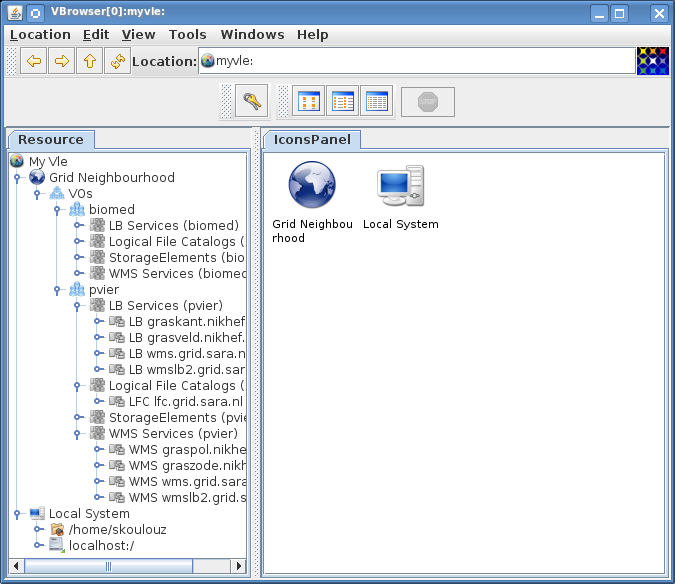
\includegraphics[scale=0.5]{vbrowser_main}}
 \caption{VBrowser window}
 \label{fig:vbrowser_window}
 \end{figure}
 
 
\subsubsection{Resource Tree panel} 
\label{section:resourcetree_panel}
 In the ResourceTree (Figure \ref{fig:vbrowser_window} left panel) in the upper 
 left there is the main resource or root resource called \myvle\ (You can rename 
 this resource). Directly below \myvle\ you can see the \GridHood\ containing 
 your VOs and the resources associated with them (see Section \ref{GridHood}). 
 Under that there is the \LocalSys\ with your home directory. All the resources in 
 this tree represent a logical ordering of your resources. When clicking on a tree 
 node the VBrowser will connect to the remote server or resource and 'open' the 
 location. If the user doesn't click on the node or expands the tree the remote 
 server or resource will not be opened and no connection is used. Some actions might 
 require that the user first has opened the resource. 
 \\

\subsubsection{Icons panel} 
\label{section:icons_panel}
 The icons panel is by default the panel you see on the right when starting the
 \vbrowser.


\subsubsection{Actions}  
 Double click (Action Click) on the resources (their icons) to open these
 location or right click (or use alternative mouse button) to view and/or edit the properties of
 these resources. 
\par
 You can add new resources by right-clicking (or use alt-mouse-button)  on
 \myvle\ and select \Menu{new}. This also works by right clicking
 (alt-mouse-button) on the white space between the icons or \emph{canvas} in
 the IconsPanel on the right. 
\\

\subsubsection{Menu Bar}
The menu bar has six menus: 
\begin{itemize}
  \item \Menu{Location}. This includes sub-menus like New Window, Open, Close, etc.
  \item \Menu{Edit}, with cut, copy, paste, etc.
  \item \Menu{View}. This includes sub-menus like \Menu{View as Icons} or \Menu{List}, and \Menu{Preferences}. With the \Menu{Preferences} sub-menu the user can change between single and double click mouse behaviour.
  \item \Menu{Tools} which contain the VLTerm, a terminal for SSH and bash sessions (see Section \ref{section:vlterm}) as well as some external tools.
  \item Finally there is \Menu{Windows} and \Menu{Help} used to close wind getting help and debug respectively.
\end{itemize}
 
\subsection{Location and navigation bar}
\label{section:location_bar}

 The location bar is the place or location which you are currently viewing. It
 has standard navigation buttons like \emph{Back}, \emph{Forward}, \emph{Up} and
 \emph{Refresh}. 
 
  \begin{figure}[htbp]
  \centerline{
\includegraphics[scale=0.5]{locationbar}}
  \caption{Location bar}
  \label{fig:locationbar}
  \end{figure}

You can drop icons and other URLs (or URI compatible strings) into this
location. For example you can drag windows icons (from your windows desktop) and
internet browser links (from for example Internet Explorer or Firefox) into this
location bar. 
Also you can start a drag from the mini icon in the location bar and drop
resources into the ResourceTree, IconsPanel or on your native desktop. 
The action of a VBrowser to native desktop Drag and Drop (DnD) might depend
how your local operating settings are configured. \\
You can also drag files directly from your local desktop into the ResourceTree
and IconsPanel windows. 
\\
\subsubsection{Navigation Buttons}

Here is an overview of the navigation buttons:

 \begin{itemize}
  \item  
\includegraphics[scale=0.5]{refresh_icon} 
	Refreshes the current viewed location. 
  \item  
\includegraphics[scale=0.5]{browse_back_icon}
    Browses back one location from history.
  \item  
\includegraphics[scale=0.5]{browse_forward_icon}
    Browses a location forward again, when the user has browsed back.
  \item  
\includegraphics[scale=0.5]{browse_up_icon}
   Browse to the parent location of the current viewed location. 
   
 \end{itemize}
 
\subsection{Toolbars}
\label{section:toolbars}

 Toolbars are the bars which have a set of buttons with small icons in them. 
 These buttons represent menu shortcuts or optional ways to view the contents
 of a location. 

  \begin{figure}[htbp]
  \centerline{
\includegraphics[scale=0.5]{toolbar}}
  \caption{Toolbars in the VBrowser}
  \label{fig:toolbars}
  \end{figure}

 An overview of the current toolbar buttons is as follows: 
 
 \begin{itemize}
 \item  
\includegraphics[scale=0.5]{invalid_creds_icon}
   Grid Credentials button. Status is invalid: Grid proxy has not been
   created.
 \item  
\includegraphics[scale=0.5]{valid_creds_icon}
    Grid Credentials button. Status is valid: Grid proxy has been created.
 \item  
\includegraphics[scale=0.5]{icons_icon}
   Icons panel button.
 \item  
\includegraphics[scale=0.5]{list_icon}
   List panel button. 
 \item  
\includegraphics[scale=0.5]{table_icon}
   Table panel button. 
\end{itemize}
  
Pressing the icon button will show the resources as icons, pressing the table
icons will present the resources in table with detailed information about the
resources. 

\subsection{Table panel}
\label{section:table_panel} 

When clicking on the table panel icon details from the resources will be
shown in a table form as can be seen in Figure  \ref{fig:table_panel}. 

\begin{figure}[htbp]
\centerline{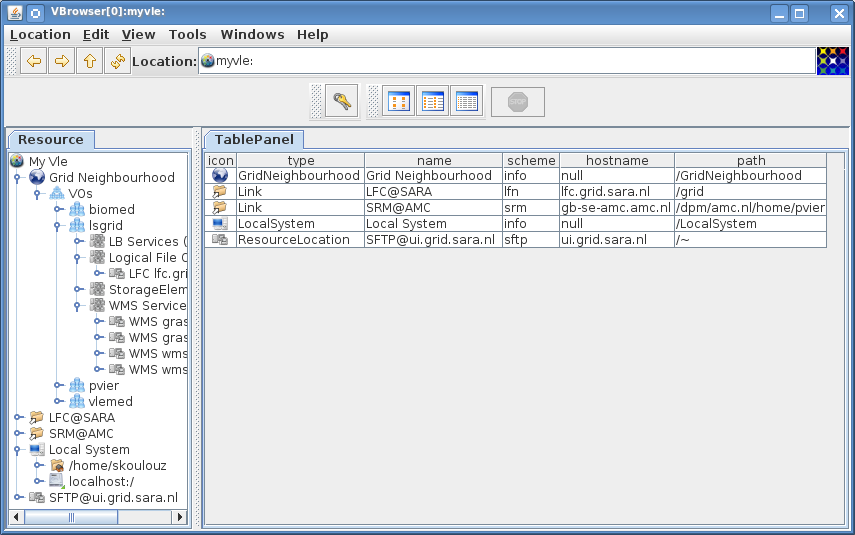
\includegraphics[scale=0.5]{table_panel}}
\caption{Table Panel}
\label{fig:table_panel}
\end{figure}

For each resource the default attributes are shown. 
Clicking on the header of the table column will sort the table according to the
logical value of the fields in that column. \\
More attributes can be added by right-clicking (or pressing alt-mouse button) on
the headerbar of the table panel as can be seen in 
Figure \ref{fig:table_panel_add_attributes}.\\


\begin{figure}[htbp]
\centerline{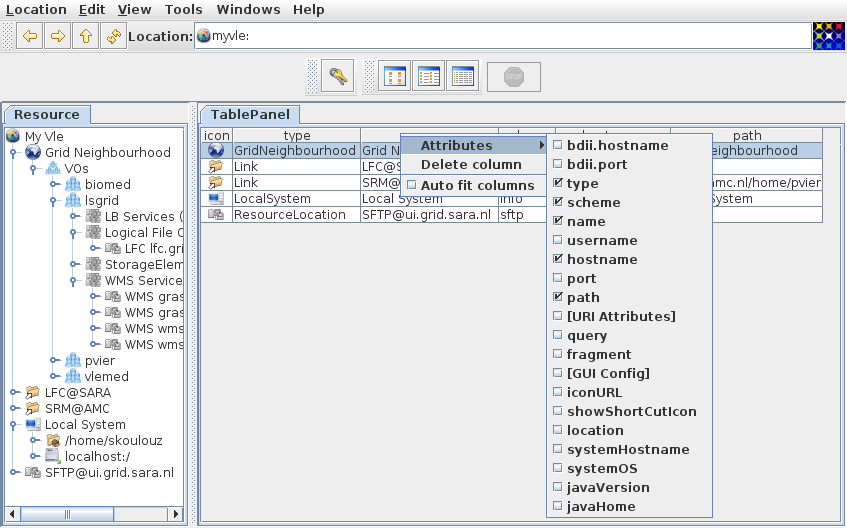
\includegraphics[scale=0.5]{table_panel_add_attributes}}
\caption{Table Panel with Attributes menu}
\label{fig:table_panel_add_attributes}
\end{figure}

You can also move around the columns by dragging the column header to the 
desired position. 
Currently the layout of the table is not saved between browsing sessions. 

\subsection{Pop-up or Action menu}

When right-clicking (or use alternative mouse button) on a resource, an pop-up
menu will appear. This is the Resource's Action Menu and from this menu special
actions can be selected which are to be performed on the resource. 
These actions include standard \Menu{Copy} and \Menu{Paste} actions as well as 
more complicated actions. See Figure \ref{fig:vbrowser_action_menu}

 \begin{figure}[htbp]
  \centerline{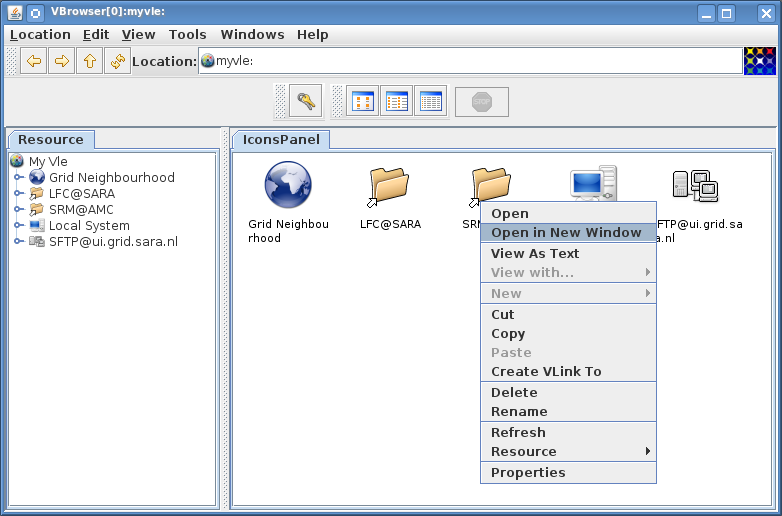
\includegraphics[scale=0.5]{vbrowser_action_menu}}
  \caption{VBrowser Action Menu}
  \label{fig:vbrowser_action_menu}
 \end{figure}
  
 \section{Authenticating yourself with the Grid} 
 \label{section:auth}

The first thing you do is to authenticate yourself with the grid. This is done
by creating a \Emph{grid proxy certificate} which is a file containing a temporary key which
you must use to access resources on the grid. 
For security reasons this file can only be used for a limited time. \\
To create a grid proxy you can use your \Emph{Grid Certificate} and your secret
\Emph{Passphrase} which combined can create a Grid Proxy for you. \\
To create one interactively,  click on the \Emph{keys} icon which can be seen in
Figure \ref{fig:grid_proxy_icon}. 

 \begin{figure}[htbp]
  \centerline{
\includegraphics[scale=0.5]{invalid_creds_icon}}
  \caption{Grid Proxy Icon}
  \label{fig:grid_proxy_icon}
 \end{figure}

A dialogue will appear where you can create your grid proxy. See Figure: 
\ref{fig:grid_proxy_init_dialog}. 

 \begin{figure}[htbp]
  \centerline{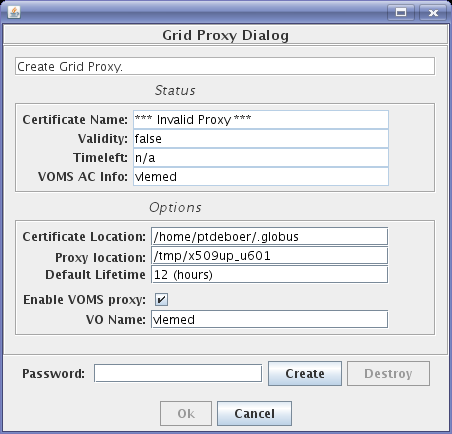
\includegraphics[scale=0.5]{grid_proxy_init}}
  \caption{Grid Proxy Creation Dialogue}
  \label{fig:grid_proxy_init_dialog}
 \end{figure}

To create a Grid Proxy, enter your passphrase and press \Menu{Create}. Your
grid proxy will be valid for 12 hours if not specified otherwise. Also to be 
able to use resources assigned to your VO, you would have to enable the 
\Menu{VOMS proxy}\footnote{VO: Virtual Organization. VOMS: Virtual Organization 
Management Service} option and fill in your VO name. More information about 
VOs may be found here: \cite{foster:2001:grid-anatomy,springerlink:10.1007/978-3-540-24689-3_5}
You can enter grid proxy creation options, like proxy location (file path) and
lifetime (in hours), in the dialog if needed. Also you can \Menu{Destroy} 
your grid proxy if you don't need it any more. Pressing \Menu{Create} again will 
refresh your proxy and update it with a new lifetime.\\

\section{Grid Neighbourhood}
\label{section:grid_hood}
 The \GridHood\ is a collection of Grid Resources (File Catalogue,Storage Elements,etc.) 
 grouped by VO. It can be configured using the property panel specifying the host and port of the BDII 
 service to query \cite{cite:bdii,cite:gridinfo}. 

 \begin{figure}[htbp]
  \centerline{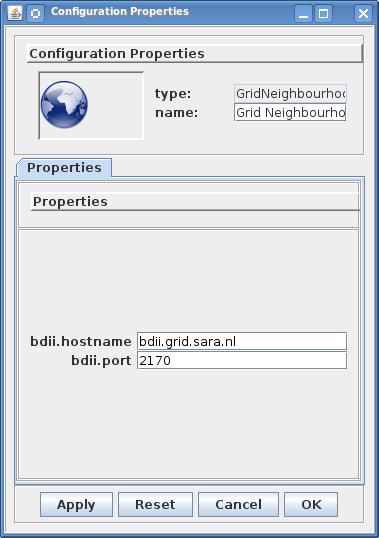
\includegraphics[scale=0.5]{gridHood_properties}}
  \caption{\GridHood\ properties}
  \label{fig:gridHood_properties}
 \end{figure}

 This resource seen in Figure \ref{fig:grid_hood} is organized as following: 
\begin{itemize}
  \item \GridHood\ . The top level resource.
  \item \VOGroup\ . The collection of VOs the user is part of. Each time the user authenticates 
                    him self having the \Menu{VOMS proxy} enabled, a new \VOGroup\ is created. 
                    Alternatively the user can create a new \VOGroup\ manually, by pressing \rightclick\ ,
                     \Menu{New}, \Menu{VO}. Moreover the current active VO is indicated with a different 
                     icon (see Figure \ref{fig:selected_vo_icon}).
  \item \VO\ . The collection of resources that this VO has at its disposal.
\end{itemize} 

 \begin{figure}[htbp]
  \centerline{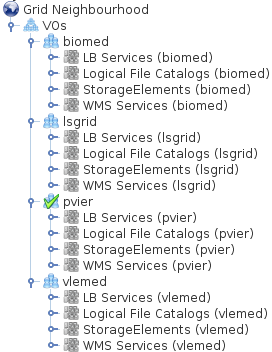
\includegraphics[scale=0.5]{grid_hood}}
  \caption{\GridHood\ Resource hierarchy}
  \label{fig:grid_hood}
 \end{figure}

%%
%% Note: selected_vo_icon is larger (128 pixels) then other (48 pixel)
%% 
 \begin{figure}[htbp]
  \centerline{
\includegraphics[scale=0.25]{selected_vo_icon}}
  \caption{The icon for the selected VO}
  \label{fig:selected_vo_icon}
 \end{figure}
 
Section \ref{section:configuring_myvle} describes how to add more resources, that might not be published by the BDII service as well as how to customise resource settings.

\section{Configuring your personal environment}
\label{section:configuring_myvle}

 When the \vbrowser\ starts, the left panel will show the Resource Tree with
 as first entry the 'Root Resource' currently named:  \myvle. 
 This root resource will contain your personal grid environment. You can rename
 this 'Toplevel Resource' to your any name you want. 

\subsection{Adding Resources} 
\label{section:adding_resources} 

 To add resource to your root resource, do the following:

	\step \rightclick\ on \myvle\ and select:\Menu{New}
	
	\step Select the resource you want to add. 


 \begin{figure}[htbp]
 \centerline{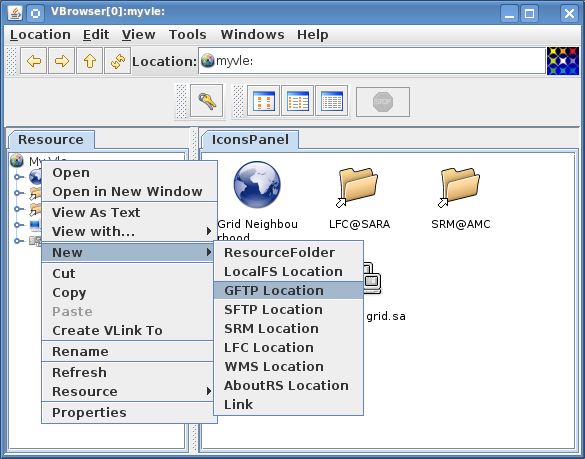
\includegraphics[scale=1]{myvle_new_server}}
 \caption{Create new location}
 \label{fig:myvle_new_server}
 \end{figure}

Deleting can be done as follows:\\
\\
\step \rightclick\ on the resource icon you want to delete and 
select:\Menu{Delete}\\ 
\\
\Note{Note}: Deleting a resource from the root resource (\myvle) will delete
the entry, never the directory it points to.\\
\\
To configure the settings for a resource, select the properties from the
pop-up menu as follows:\\
\\
\step \rightclick\ on the resource icon and select:\Menu{properties}\\
\\
Check and optionally change the properties of this resource.
	
\subsection{Adding New (Grid) Resource Location} 
\label{section:adding_gftp_server}
 
You can add a new Grid Resource Location, for example a 'GridFTP' location as
follows:\\
\\
\step \rightclick\ on \myvle\ and select:\Menu{New} \rarr \Menu{GFTP Location}\\
\\
Now set the GridFTP Location by selecting the properties
option from the pop-up menu as follows: \\
\\
\step \rightclick\ on the GridFTP icon and select:\Menu{properties}\\
\\
\begin{figure}[htbp]
\centerline{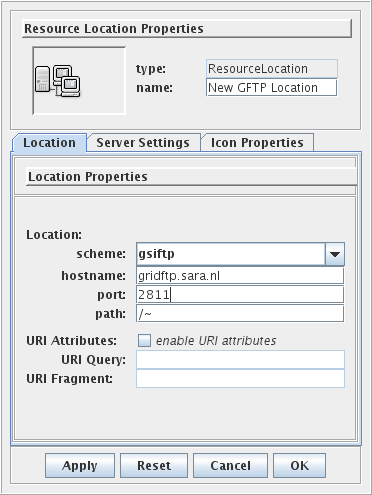
\includegraphics[scale=1]{gftp_location}}
\caption{GridFTP Location}
\label{fig:gftp_location}
\end{figure}
\\
Fill in the location of the new GridFTP server.
\\
\begin{itemize}
\item \Emph{scheme} : the scheme to use. For GridFTP leave this to 'gsiftp'.
\item \Emph{host}  : the hostname of the GridFTP location. 
\item \Emph{port}  : the port of the GridFTP location. The default value is
'2811'
\item \Emph{path}  : The path to start browsing. Leave to '$\sim$' to use
your default home location on the remote server. 
\item \Emph{URI properties}  : Not supported for GridFTP. 
\end{itemize}

To configure the server properties for this location, click on the \Menu{Server
Settings} tab and specify the settings for this server. 
\\
\begin{figure}[htbp]
\centerline{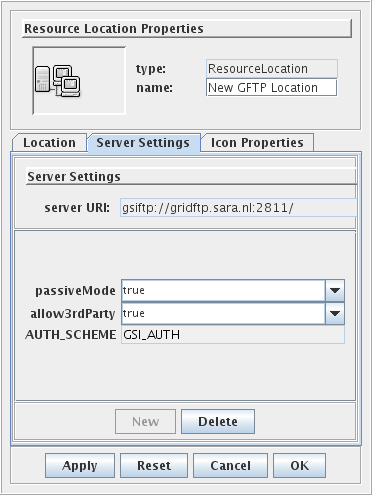
\includegraphics[scale=1]{gftp_properties}}
\caption{GridFTP Server Settings}
\label{fig:gftp_properties}
\end{figure}
\\
Current Server Settings for GridFTP servers are:
\begin{itemize}
\item \Emph{passiveMode} : set to 'true' when incoming connections are not
possible, for example when browsing from behind a firewall. 
\item \Emph{allow3rdParty} : whether 3rd party copying is possible to and from
this server.  This is used when copying between two (remote) Grid FTP locations.  
\end{itemize}

\subsection{Adding an LFC Location} 
\label{section:adding_lfc_server} 

To create an LFC \cite{10.1109/HPDC.2005.1520941} location do as follows:

	\step \rightclick\ on \myvle\ and select:\Menu{New} \rarr \Menu{LFC
	Location}

 After creating a new location the resource properties editor should pop-up. 
 You can also manually edit these properties by selecting the edit properties
 option from the pop-up menu as follows: 

	\step \rightclick\ on the LFC icon and select:\Menu{properties} 

\begin{figure}[htbp]
\centerline{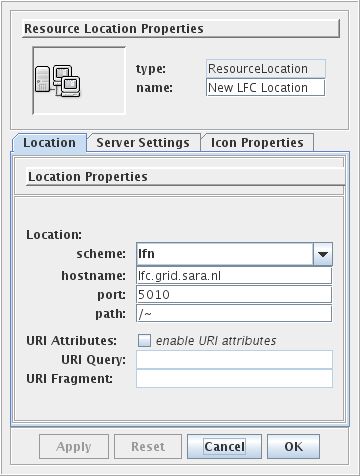
\includegraphics[scale=1]{lfc_location}}
\caption{LFC Location}
\label{fig:lfc_location}
\end{figure}

Fill in the location of the new LFC server.

\begin{itemize}
\item \Emph{scheme} : the scheme to use. For LFC leave this to 'lfn'.
\item \Emph{host}  : the hostname of the LFC server. 
\item \Emph{port}  : the port of the LFC server. The default value is '5010'
\item \Emph{path}  : the path to start browsing. Fore example '/grid/lsgrid' or 
                     use tilde: '$/\sim$' to auto resolve to you VO home location. 
                        
\item \Emph{URI properties}  : Not supported for LFC locations.  
\end{itemize}

 \begin{figure}[htbp]
  \centerline{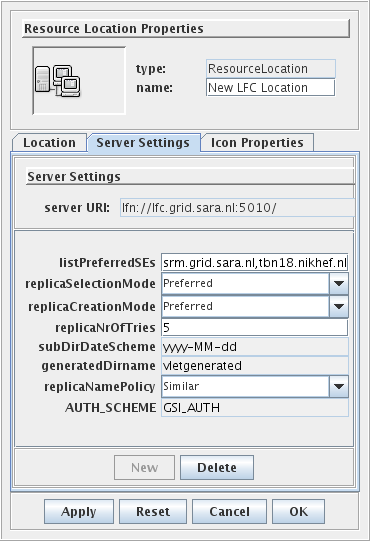
\includegraphics[scale=1]{lfc_properties}}
  \caption{LFC Server Settings}
  \label{fig:lfc_properties}
 \end{figure}

To specify the server configuration for this location, click on the
\Menu{Server Settings} tab and specify the settings for this server. 
Here an overview of the LFC settings:

\begin{itemize}
\item \Emph{listPreferredSEs} : list of Preferred Storage Elements to
use when selecting a replica to read from or when creating a new replica. This
is a comma seperated list of hostnames which can have an optional port number. 
\item \Emph{replicaSelectionMode} : replica selection algorithm used when
there is more then one replica to choose from (used when reading an
LFC file).
\item \Emph{replicaCreationMode} : Storage element selection algorithm
used when creating new replicas (used when uploading or writing to an LFC file). 
\item \Emph{replicaNrOfTries} : number of attempts tried when selecting a
replica to read from or when creating a new replica at a Storage Element. A
minimum of 3 is recommend or the number of replicas+1 if that if bigger than 3.     
\item \Emph{generatedDirname} : parent directory which will be used
at a Storage Element for all generated replicas. This directory name will be
appended to the default VO writeable location or VO Storage Area (see
explanation below).
\item \Emph{subDirDateScheme} : sub directory syntax used when
replicas are created in the replica parent directory: \Emph{generatedDirname}
(see explanation below).
\item \Emph{replicaNamePolicy} : file name policy when creating replicas at
Storage Elements (see explanation below). 
\end{itemize}

Each of the above server properties is explained more in details below: 

\subsubsection{List of Preferred Storage Elements (listPreferredSEs) } 

The server property \Emph{listPreferredSEs} is a comma seperated list of
hostnames which contains the user preferred Storage Elements. 
This list is used when uploading a file to an LFC server to choose a
Storage Element to store a replica.  
When downloading a file, this list is used to select a replica witch matches a
Storage Element from this list. How this matching occurs depends on 
the \Emph{replicaSelectionMode} or the \Emph{replicaCreationMode} settings.    

\subsubsection{Replica Selection Algorithm (replicaSelectionMode) } 

The option \Emph{replicaSelectionMode} determines which algorithm is used when
selecting a replica to read from. This is one of the following: 

\begin{itemize}
  \item \Emph{Preferred}$^1$ :  Try to find a replica which matches one of the
  hostnames listed in the server property which specified the list of preferred
  Storage Elements: \Emph{listPreferredSEs}. 
  The order in which replicas are tried is the same as the order of the
  hostnames in this list. 
  \item \Emph{PreferredRandom}\footnote{} : Same as \Emph{Preffered} but the list of
  matching replicas is randomized. 
  \item \Emph{AllSequential} : Try all replicas in order as they are registered
  at the LFC server. The first that is available will be used. If all replicas
  have been tried, the selection procedure will start with the first until the
  maximum number of tries has been reached. 
  \item \Emph{AllRandom} : Same as \Emph{AllSequential} but the order in which
  replicas are tried is randomized. As this randomization is 'true' random,
  same replicas might be tried twice in a row. This is by design. 
\end{itemize} 

\Note{$^1$} If no replicas match the list of preferred Storage Elements
(\Emph{listPreferredSEs}) or this list is empty, the mode \Emph{AllSequential}
will be used.

\subsubsection{Replica Creation Algorithm (replicaCreationMode) }

The option \Emph{replicaCreationMode} determines which algorithm is used when
selecting a Storage Element to create a replica. 
This is one of the following:

\begin{itemize}
  \item \Emph{Preferred} :  Only the Storage Elements from the 
      \Emph{listPreferresSEs} list are use to create a new Replica. The order in
      which Storage Elements are tried is the same as the order of the list. 
  \item \Emph{PreferredRandom} : Same as \Emph{Preferred} but the list will be
      randomized. Since the randomiser is 'true' random, a Storage Element
      might be tried multiple times even if it has already been tried before
      unless it already has a replica. 
  \item \Emph{DefaultVORandom} : A Random Storage Element is used from the list
  of allowed Storage Elements for the current user's VO by querying the grid info
  service (BDII). If this Storage Element fails another is randomly selected.   
\end{itemize} 
 
\subsubsection{Replica number of Tries (replicaNrOfTries) } 

The number of attempts undertaken to either read a replica or the number of
attempts to create a replica at a Storage Element. 

\par
When reading from an LFC file (downloading), this number determines how many
times an attempt is made to read from any of the available replicas.
If, for example, the number of replicas is only 1, the same replica will be
tried each time. 
If the number of available replicas is less than the \Emph{replicaNrOfTries} the
same replica might be tried more then. Which replica is used depends on the
\Emph{replicaSelectionMode}.

\par
When uploading a file to LFC, this number determines how many times an
attempt is made to create a replica at one of the available Storage
Elements. Which Storage Element is used depends on the
\Emph{replicaCreationMode}.

\subsubsection{Replica directory and file name creation policy
(generatedDirname, subDirDateScheme, replicaNamePolicy) }

The options \Emph{generatedDirname}, \Emph{subDirDateScheme} and 
\Emph{replicaNamePolicy} determine which path is used when creating a replica
at a Storage Element.\\
The path is created by using the following syntax:\\
\\
\Path{ srm://\lt VO Storage Area\gt /\lt generatedDirname\gt/\lt
subDirDateScheme\gt/\lt replicaFileName\gt}\\
\\ 
The \Path{ \lt VO Storage Area\gt} is the VO allowed Storage Area which is
dynamically determined by querying the appropriate grid info service (BDII). 

The \Path{\lt replicaFileName\gt} is a generated file name which can resemble
the logical file name of the LFC entry the file is an replica for. This depends
on the \Emph{replicaNamePolicy} setting. \\
This can be one of the following:

\begin{itemize}
  \item \Emph{Random} : The filename is a randomized file name only.  
  \item \Emph{Similar} : The filename contains the original logical filename
  and a randomized identifier. 
\end{itemize}

Example of a \Emph{Random} replica file path at a storage element:\\
\\
\tab
\Path{
/pvier/vletgenerated/2009-07-01/file\_fad71348-d80b-48e5-bf2d-24590bb7c5f2
}
\\
\\
Example of a \Emph{Similar} replica file path for the LFC file with name
'experiment.txt' :\\
\\ 
\tab
\Path{ /pvier/vletgenerated/2009-07-01/experiment\_txt\_fad71348-d80b-48e5-bf2d-24590bb7c5f2
}
\\

% \subsection{Adding an SRB Location} 
% \label{section:adding_srb_server} 
%  To create an SRB location perform the following steps: 
%  
% 	\step \rightclick\ on \myvle\ and select:\Menu{New} \rarr \Menu{SRB
% 	Location}
% 
%  Now set the SRB location properties by selecting the properties option
%  from the pop-up menu as follows: 
%  
% 	\step \rightclick\ on the SRB icon (MySRB) and select:\Menu{properties}  
% 
%  \begin{figure}[htbp]
%   \centerline{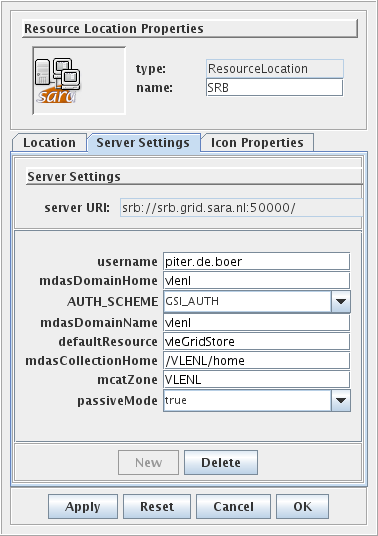
\includegraphics[scale=0.5]{srb_properties}}
%   \caption{SRB server properties}
%   \label{fig:srb_properties}
%  \end{figure}
% 
% Current Server Settings (Select the \Menu{Server Settings}  tab) for SRB servers
% are:
% \begin{itemize}
% \item \Emph{passiveMode} : set to 'true' when incoming connections are not
% possible, for example when browsing from behind a firewall. 
% \item \Emph{AUTH\_SCHEME} : authentication scheme. GSI authentication is the
% standard used on the Grid. 
% \item \Emph{mdas/mcat settings} : Make sure you fill in the right
% \Emph{mdas}\ldots settings and \Emph{mcat}\ldots settings. Contact your SRB
% administrator for the right values. 
% \item \Emph{defaultResource} : A SRB Server might allow different values
% for the \Emph{defaultResource}. Contact your SRB administrator for the right
% values. (Values given are example values).
% \end{itemize}


\section{Links or shortcuts}
\label{section:links} 

 Another way of creating a resource entry is creating a \link. A \link\ behaves in
 a similar way as shorcuts on windows. This type of resource does \Emph{not} 
 resemble a Unix hard- of softlink in anyway. When opening a \link, the location 
 pointed to by the \link, will be opened. 
 
 Typically a \link\ icon has a small arrow in the bottom left corner
 to indicate it is a link, as can be seen in Figure \ref{fig:linkicon}.

 \begin{figure}[htbp]
  \centerline{
\includegraphics[scale=0.5]{linkicon}}
  \caption{Link icon}
  \label{fig:linkicon}
 \end{figure}

 You can create a link by selection the \Menu{Create VLink to} option from 
 the pop-up menu or action menu. 
\newpage

%% Chapter 3 
%
% VBrowser
%

\chapter{Other Tools}
\label{chap:other_tools}

\section{Application and Tools} 

Other applications currently available in the VL-e Toolkit are:

\begin{itemize}
  \item \Bold{GridProxyDialog}: for creating and managing Grid Proxies. 
  \item \Bold{VLTerm}:		    simple vt100 emulator with some
  xterm extensions.  
  \item \Bold{uricopy.sh,urils.sh}:		URI copy and list script. 
  \item \Bold{jython.sh}:		Jython startup script. 
\end{itemize}

\section{GUI utils}

\subsection{GridProxyDialog}

Some part of the \vbrowser\ can be used stand alone. 
The Grid Proxy Init dialog can be called by running the
\Path{GridProxyDialog.jar} as follows:\\

	\tab \Code{java -jar \$VLET\_INSTALL/bin/GridProxyDialog.jar}\\

Or double click on the jar file in the \Path{VLET\_INSTALL/bin} directory:\\

	\tab \Path{VLET\_INSTALL/bin/GridProxyDialog.jar}\\
	
You cannot move this file out of the installation, but you can create a shortcut
to the jar file instead. 

\subsection{VLTerm}
\label{section:vlterm}

The VL-e Toolkit has an beta version of a VT100 terminal emulation program.
This terminal emulator can be used as a backup if there is no standard xterm or SSH
terminal program available on the user's host.\\
Most VT100 and some XTERM control codes are supported. For basic remote
command execution this terminal application can be used.\\
To start the \Code{VLTerm} application use the command line as follows:\\

	\tab \Code{java -jar \$VLET\_INSTALL/bin/vlterm.jar}\\

Or double click on the jar file at the following path:\\

	\tab \Path{VLET\_INSTALL/bin/vlterm.jar}\\

You cannot move this file out of the installation, but you can create a
shortcut to the jar file instead. \\ 

 \begin{figure}[htbp]
 \centerline{\includegraphics[scale=0.75]{vlterm}}
 \caption{VLTerm at SARA}
 \label{fig:vlterm}
 \end{figure}

\section{Command line tools}

\subsection{URI copy script: uricopy.sh}

At this moment there is only one script interface to the Virtual Resource System
(VRS). This script is the URI copy script: \Path{uricopy.sh}\\

The location is: \Path{VLETINSTALL/bin/uricopy.sh} and the syntax is as
follows: 

\tab \Path{uricopy.sh [options] \lt source URI\gt\ \lt destination URI\gt\
	[-D\lt PROPERTY\gt =\lt VALUE \gt]*}

Command line argument are: 
\begin{itemize}
  \item \Path{  \lt source URI\gt\ } : source file or directory.
  \item \Path{  \lt dest URI\gt\ } : parent directory to copy to. The source
        file  or directory is always created as child of this parent
        directory.
  \item \Path{ [options] } can be: 

\hspace*{10mm}\begin{minipage}{170mm}
\begin{verbatim}
 -r,-dir    ; perform a recursive copy of the source location (for copying 
              directories). 
 -v [-v]    ; be verbose. provide option twice to be even more verbose. 
 -f, -force ; overwrite (optional) existing target location. 
 -move      ; move resource and delete source URI after copy command.
 -mkdirs    ; create target directory path 
 -result    ; print resulting destination URI as follows: "result=...".
 -debug     ; enable debug output.
\end{verbatim}
\end{minipage}
\end{itemize}

The properties which can be specified are depending on the source and
destination URIs. Most VLET settings can be specified as command line options 
using the \Code{-D\lt NAME\gt =\lt VALUE\gt} syntax. \\
\\
An overview of relevant properties are:\\
\\
\EmphBold{Global properties}:\\
\\
\tab \Code{-DpassiveMode=true} always use passive mode for all file transfers.\\
\\ 
\EmphBold{General usage:}\\
\\
The source and destination URIs are mandatory. Options can be both specified
before and after the URIs. The source URI must be an existing file or directory
and the target URI \Emph{must} be an existing directory! This is to
avoid ambiguity between destination files and directories. The new file or
directory will always be created as a child entry in the target directory.\\
\\
\EmphBold{Copying directories:}\\
\\
To copy a directory specify the \Code{-r} option (for recursive copy).\\
The uricopy command will create the new destination directory which
always will be a child (subdirectory) of the destination URI.\\
\\
\EmphBold{Moving files or directories:}\\
\\
To move a file or a directory specify the \Code{-move} option. The source will
be deleted after and \Emph{only} after a successful copy. \\
\\

\subsection{Examples} 

\subsubsection{LFC uricopy example}

Below an example how to use uricopy to upload a file to an LFC server. 

\hspace*{10mm}\begin{minipage}{170mm}
\begin{verbatim}
$VLET_INSTALL/bin/uricopy.sh file:/home/ptdeboer/hello.txt \
	lfn://lfc.grid.sara.nl/grid/pvier/piter
\end{verbatim}
\end{minipage}

Options or server settings can be provided as either a Java property or a URI
attribute. \\
For example to specify the preferred Storage Elements provide the
\Emph{lfc.listPreferredSEs} option to the uricopy script:\\

\hspace*{10mm}\begin{minipage}{170mm}
\begin{verbatim}
$VLET_INSTALL/bin/uricopy.sh file:/home/ptdeboer/hello.txt \
	lfn://lfc.grid.sara.nl/grid/pvier/piter\
	-Dlfc.listPreferredSEs=srm.grid.sara.nl,tbn18.nikhef.nl
\end{verbatim}
\end{minipage}

The above command will try to register the file at the first Storage Element in
the list, if that fail it will try the second storage element. 

Optional LFC properties can be: \\

\hspace*{10mm}\begin{minipage}{170mm}
\begin{verbatim}
-Dlfc.listPreferredSEs=SEHost1,SEHost2 ; list of preferred Storage Elements
-Dlfc.replicaNrOfTries=5               ; number of retries when reading/creating
                                         a replica. 
-Dlfc.replicaCreationMode=Preferred    ; one of: Preferred, PreferredRandom,
                                         DefaultVO, DefaultVORandom 
-Dlfc.replicaSelectionMode=Preferred   ; one of: Preferred,PreferredRandom,
                                         AllSequential, AllRandom
\end{verbatim}
\end{minipage}\\

% \subsubsection{SRB uricopy example}
% 
% An example how to upload files to the SRB server goes as follows:
% 
% \hspace*{10mm}\begin{minipage}{170mm}
% \begin{verbatim}
% $VLET_INSTALL/bin/uricopy.sh file:/home/ptdeboer/hello.txt \
%    srb://srb.grid.sara.nl:50000/VLENL/home/piter.de.boer.vlenl \
%    -Dsrb.defaultResource=vleGridStore \
%    -Dsrb.username=piter.de.boer \
%    -Dsrb.msdasDomainName=vlenl
% \end{verbatim}
% \end{minipage}
% 
% Optional SRB properties can be: \\
% 
% \hspace*{10mm}\begin{minipage}{170mm}
% \begin{verbatim}
% -Dsrb.username=USERNAME               ; username for the SRB server.
% -Dsrb.defaultResource=vleMatrixStore  ; specify resource to store new file/directories.
% -Dsrb.mdasCollectionHome=/VLENL/home  ; specify default home.
% -Dsrb.mdasDomainName=vlenl            ; specify DomainName.
% -Dsrb.hostname=srb.grid.sara.nl       ; hostname of SRB server.
% -Dsrb.port=50000                      ; port of SRB server.
% \end{verbatim}
% \end{minipage}\\
% 
% If you specify any of the above as command line options, you can omit them in the
% URI. \\
% The option:\\
% \\
% \tab \Code{-Dsrb.defaultResource=vleGridStore}\\
% \\
% may be omitted if the default resource of the SRB server
% (\Code{(srb.defaultResource}) equals the one specified in srb settings file:
% \Path{VLETINSTALL/etc/srbsettings.prop.}\\
% If this option is not or incorrectly set the SRB server might return an error as
% follows:\\
% \\
% \hspace*{10mm}\begin{minipage}{170mm}
% \begin{verbatim}
% 	OBJ_ERR_RES_NOT_REG resource has not been registered -2400
% \end{verbatim}
% \end{minipage}
% 
% This means the SRB server could not 'register' the file at the default 'storage'
% location.\\
% \\
% \EmphBold{SRB upload example using URI attributes}:\\
% \\
% Used URIs can have (URI) attributes which allow Server Properties and Settings
% to be specified as part of the URI.\\
% Check the implementation details, or see in the appendices, which property is
% supported as URI attribute.\\
% An example is as follows:\\
% \\
% \hspace*{10mm}\begin{minipage}{170mm}
% \begin{verbatim}
% $VLET_INSTALL/bin/uricopy.sh file:///home/ptdeboer/hello.txt
%    srb://srb.grid.sara.nl:50000/home/piter.de.boer.vlenl\
%    ?srb.defaultResource=vleGridStore\
%    &srb.username=piter.de.boer\
%    &srb.mdasDomanName=vlenl
% \end{verbatim}
% \end{minipage}\\
% \\ 
% \\
% The difference is that the defaultResource property is now specified as URI
% attribute using the \path{?srb.defaultResource=vleGridStore} syntax. \\
% \\
\subsection{Customized uricopy script}

You can use the uricopy.sh as an example and modify it to your liking. Make sure 
the \VLETINSTALL environment variable is set so the script can find the
installation as follows: \\
\\
\hspace*{5mm}\begin{boxedminipage}{165mm}
\begin{verbatim}

#!/bin/bash 
##
# File   : Example modified uricopy.sh script 
# Version: VLET 1.1
# --- 

# Default installation: 
export VLET_INSTALL=/opt/vlet
export VLET_SYSCONFDIR=$VLET_INSTALL/etc
# Configuration files on PoC R3: 
#export VLET_SYSCONFDIR=/etc/vlet

# set base directory 
BASE_DIR=$VLET_INSTALL

# my options: 
OPTIONS="-DpassiveMode=true -Dsrb.username=piter.de.boer -r -force"

# source vlet settings: 
source $VLET_SYSCONFDIR/vletenv.sh 

##
# VLET java class to start: VFSCopy 
CLASS=nl.uva.vlet.vfs.VFSCopy

# JVM options: 
JVMOPTS="-Dvlet.install.sysconfdir=$VLET_SYSCONFDIR -jar $BASE_DIR/bin/bootstrapper.jar"

# Start bootstrapper which does the rest 
echo "Command:" $JAVA $JVMOPTS $CLASS $OPTIONS $@
$JAVA $JVMOPTS $CLASS $OPTIONS $@
# keep return value: 
RETVAL=$? 

#return exit code from VFSCopy
exit $RETVAL; 

\end{verbatim}
\end{boxedminipage}

\section{Jython}

\subsection{Jython start script: jython.sh}

Since Jython is a pure java implementation of Python, Jython can be used 
to access to full VLET API. To run  a Jython script, call the Jython 
bootstrap script from the VLET installation. \\
The location of this bootstrap script is: \Path{VLETINSTALL/bin/jython.sh} and
the syntax is as follows: \\
\\
\tab \Path{jython.sh [-i] \lt jython file\gt\ }\\
\\
Where option \Path{-i} starts the Jython interpreter in interactive mode (leave
out the file when starting the Jython interpreter in this mode). \\
Jython examples can be seen in: \Path{VLETINSTALL/py}. 
\\
The documentation for the VLET API can be found at: 
\Path{VLETINSTALL/doc/api/index-all.html}. \\ 
\\ 
Below an example how to use the VFS interface from VLET in a Jython 
script:

\hspace*{5mm}\begin{boxedminipage}{165mm}
\begin{verbatim}
#!/opt/vlet/bin/jython.sh
##
# VFSClient jython interface example
# (C) www.vl-e.nl 
##
# File         : vfsclient.py 
# Vlet version : 1.1
# Author       : Piter T. de Boer 
#
# Info :  
#    VLET vfs jython interface example.
#    To start execute this jython file, use:
#        $VLET_INSTALL/bin/jython.sh <jython.file> 
##
import sys
#import VRS objects + VFS Client: 
from nl.uva.vlet.vrl import VRL
from nl.uva.vlet.vfs import VFile,VDir,VFSClient

### Helper methods
def boolstr(value):
  if value == True: 
     return "true" 
  else:
     return "false" 
     
# creat new VFSClient
vfs=VFSClient()

# get Virtual File object: 
dir=vfs.getDir("lfn://lfc.grid.sara.nl:5010/grid/pvier/"); 
print "Remote LFC directory = "+dir.toString()
print "--- Directory Attributes ---" 
print " Directory modification time  =",dir.getModificationTime()
print " Directory access permissions = \""+dir.getPermissionsString()+"\"" 

#get contents of remote Directory 
contents=dir.list()

# array acces: 
print "First file = ",contents [0];

# define print function: 
def PrintNode(prefix,node):
  print prefix+"["+node.getType()+"] "+node.toString();

# apply MyPrint on contents array
print "--- contents of remote directory ---"
[PrintNode(" - ", file) for file in contents]
print "--- ---"

# get local home 
home=vfs.getDir("file:///~"); 
print "Local home=",home; 
\end{verbatim}
\end{boxedminipage}


\hspace*{5mm}\begin{boxedminipage}{165mm}
\begin{verbatim}
### remote navigation 
# get remote file:
fileVRL="lfn://lfc.grid.sara.nl:5010/grid/pvier/piter/test.txt"; 
vrlObject=VRL(fileVRL) 

# dissect VRL (=URI)
print "-- VRL object ---"
print " VRL String    =",fileVRL; 
print " VRL Object    =",vrlObject; 
print " VRL Hostname  =",vrlObject.getHostname(); 
print " VRL Port      =",vrlObject.getPort()
print " VRL Path      =",vrlObject.getPath(); 
print " VRL Extension =",vrlObject.getExtension(); 
print "---"

if (vfs.existsFile(fileVRL) is True):
  print "File exists:"+fileVRL; 
else:
  print "*** Error: Remote file does not exists:"+fileVRL; 

# get/create Virtual File object of remote file
remoteFile=vfs.getFile(fileVRL); 
print "--- File Attributes ---" 
print " modification time  =",remoteFile.getModificationTime()
print " length             =",remoteFile.getLength()
print " access permissions = \""+remoteFile.getPermissionsString()+"\"" 
print " isReadable         =",boolstr(remoteFile.isReadable()) 
print " isWritable         =",boolstr(remoteFile.isWritable()) 
print " mimetype           =",remoteFile.getMimeType()

#get contents of remote Directory 

# getContents() returns byte array, getContentsAsString returns String object 
text=remoteFile.getContentsAsString(); 
print "Contents of remote file = "+text; 

# Navigating example:  "cd .."  
remoteParent=remoteFile.getParent(); 
print "Remote parent = ", remoteParent; 

# example "VDir.hasFile()" (hasDir/hasChild)
if (remoteParent.hasFile(remoteFile.getBasename()) is True): 
   print "Remote parent reports that is has the remote file as child" 
else:
   print "***Error: Parent directory of remote file reports is doesn't have the Child!" 

# copy to local home directory, overwrite existing: 
resultFile=remoteFile.copyTo(home);
print "Copied remote file to:",resultFile; 
print "Check whether file is local:",resultFile.isLocal();
print "Local path of file is:",resultFile.getPath(); 
\end{verbatim}
\end{boxedminipage}


\hspace*{5mm}\begin{boxedminipage}{165mm}
\begin{verbatim}
# get system temp dir: 
print "tempdir'=",vfs.getTempDir(); 

# create Unique Temp Dir() on local home:
tmpdir=vfs.createUniqueTempDir(); 
print "unique tempdir =",tmpdir;

print "end."
sys.exit(0); 
\end{verbatim}
\end{boxedminipage}

See the examples directory \path{VLET_INSTALL/py/*} for more jython scripts. 
 
\newpage


%% Chapter 5
%
% VBrowser
%

\chapter{Customization}
\label{chap:customization}

\section{Custom viewers/plugins}

The VBrowser supports two kind of extension or plugins. One is for protocol 
implementations or 'VDrivers', The other are VBrowser Viewer extensions or
'Viewer Plugins'. The first are mapped to URI schemes like 'srm://' the latter
are mapped to resource mimetypes like 'text/plain'. \\
\par
You can install extra viewers or VBrowser plugins in the following directories 
(create them if they don't exist):

\begin{itemize}
  \item \Path{\VLETINSTALL/lib/plugins}: for installation plugins.
    \item \Path{HOME/.vletrc/plugins}: path for user plugins.
\end{itemize}

A \vbrowser\ plugin can be a single jar file or a directory that contains the needed
jar file and (optional) used libraries. The filename or directory must 
be the full classname of the plugin. 
This name triggers the VBrowser upon startup to load the plugin. 
For example the custom VTK image viewer which can be install at one of the
following locations:\\
\\
\tab \Path{\VLETINSTALL/lib/plugins/nl.uva.vle.app.vtk.viewer.NiiViewer/}\\
\\	
for system wide installation of custom plugins, or:\\
\\
\tab \Path{HOME/.vletrc/plugins/nl.uva.vle.app.vtk.viewer.NiiViewer/}\\
\\
for custom plugins installed for a single user only (in his or hers HOME directory). \\
\\
Some viewers might need extra configuration. For example in the case of
the above VTK viewer, specifying the VTK library paths as follows:\\
\\
\tab \Code{export LD\_LIBRARY\_PATH=\$LD\_LIBARY\_PATH:/opt/vl-e/vtk\_5.0.2/lib:/opt/vl-e/mesa3d\_6.4.2/lib}\\
\\
The above library paths are the installation paths as specified on the VL-e PoC
environment (R2). You can add them to your \Path{.bashrc} or add them to the
installation configuration in \Path{VLET\_INSTALL/etc/vletenv.sh} if library
paths are not already setup as specified. \\
\\
Extra plugins can be downloaded from the sourceforge site at the 'files'
section:\\
\\
\tab \Link{http://sourceforge.net/projects/vlet/files/}
\\

\section{Custom Mimetypes and icons}

Mimetypes are a way of telling an application what kind of content is in the
file or resource. In most cases this is a simple mapping of an extension to a 
standard defined mimetype. This mimetype is a simple string which describes 
the type of content, for example ``text/plain'' or ``image/jpeg''. Usually it
consists of a generic part (``text/'' or ``image/'') and a specific part
(``plain'' or ``jpeg'') seperated by a (forward) slash.\\ 
The following files defines the mimetypes used in \VLET:

\begin{itemize}
  \item \Path{\VLETINSTALL/etc/mime.types}: for installation configured mime
  types.
  \item \Path{HOME/.vletrc/mime.types}: for user configured mime types.
\end{itemize}

The syntax of the mimetype configuration is the mimetype name followed by a list
of extensions or complete filename(s) as follows: \\
\\
\tab \Variable{type/subtype EXT1 EXT2 EXT3\ldots}\\
\\
An example of some standard mimetypes is given as follows. First the
mimetype name is given followed by their extension(s):\\
\\
\begin{boxedlisting}[170]
\begin{verbatim}
###
# File    : mime.types
# Location: $\VLETINSTALL/etc/mime.types
# ---
# Default mime types:  <MIMETYPE>  <EXTENSION1> <EXTENSION2> ...
#

image/x-xbitmap                 xbm 
image/x-xpixmap                 xpm
image/jpeg                      jpeg jpg jpe JPG
text/rtf                        rtf
text/plain                      txt
# some custom mimetypes examples: 
application/jglite-jobids       vljids 
application/taverna-scuffle     scuffle
application/feat-fsf            fsf FSF 

#end default mime types file 
\end{verbatim}
\end{boxedlisting}

\subsection{User defined mimetypes}

A user can override the default mimetype for a resource or specify a new one  
by adding a line in the \Path{HOME/.vletrc/mime.types} file (if the file is not there the user can created) as follows:\\
\\
\begin{boxedlisting}
\begin{verbatim}
##
# File    : mime.types 
# Location: $HOME/.vletrc/mime.types
# ---
# User defined mime types 

# customized mime type for VL-e Text: 
application/vle-text      vletxt txt TXT inf info

# end user defined mime types
\end{verbatim}
\end{boxedlisting}\\
\\
Now .txt (and .TXT, .inf, .info) files will have the "application/vle-text" mimetype 
as can be seen in Figure:\ref{fig:custom_mimetypes}\\
\\
\begin{figure}[htbp]
\centerline{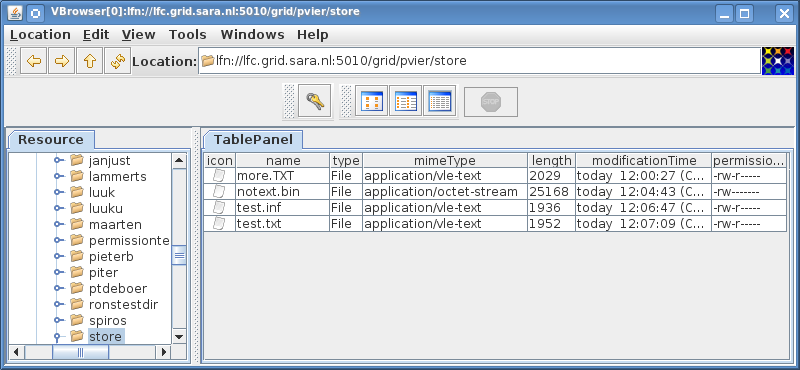
\includegraphics[scale=0.5]{vbrowser_mimetypes}}
\caption{Custom Mimetypes}
\label{fig:custom_mimetypes}
\end{figure}\\
\\
\\
\subsection{Web server mimetypes}

When browsing websites and viewing resources at web servers, the web server has the 
responsibility to return the correct mimetype for the viewed resource. 
For example an html file has the mimetype "text/html" but the URL might not always 
point to a location which ends with '.html'.
Also a query or server side script (php) might return content which differs from what 
might be expected when inspecting the URL, which for example might end in ".php". 
Configuring a web server to return custom mimetypes can be done in different ways and
is highly dependant on the used web server and (Linux) environment it runs in.\\
\\
Below configuration files for a Linux+Apache 2.0 setup: 
\begin{itemize}
  \item \Path{/etc/mime.types} Global system (Linux) mime.types file.   
  \item \Path{/etc/httpd/conf/httpd.conf} Custom HTTPD configuration file or:  
  \item \Path{/etc/apache2/httpd.conf} Custom apache 2.0 configuration file. 
\end{itemize}
 
The \Path{/etc/mime.types} follows the same syntax as described in the previous paragraph.
Changing this file will change global settings for the whole (Linux) system.\\  
\\
Below an example of extra configuration settings which can be added to the \Path{httpd.conf} file.
The location of this file depends on used web server and Linux distribution. 
See the documentation of the used web server for the correct location of this file.\\
For example, add the following custom mimetypes to the \Path{httpd.conf} file
to allow (glite) job monitoring resources to have the correct mimetype:\\
 
\begin{boxedlisting}
\begin{verbatim}
###
# Add custom VBrowser mime types. 
# Add glite jobids: 
AddType application/glite-jobids .vljids
# Add job output files ".out" and ".err" as plain text:  
AddType text/plain .out
AddType text/plain .err
\end{verbatim}
\end{boxedlisting}

After changing this file the web server needs to be restarted for the changes to have effect. 
\\ 
\\
\subsection{Magic types}
Another way to determine the file content is by matching the first bytes of a
resource with well known 'magic types' which specify the type of file. 
For example Linux executables have the letters 'ELF' in the beginning of 
the file which specifies it is an Linux Executable. \\
Other examples are: GIF files (.gif) start with the ASCII letters 'GIF' and 
WAV files (.wav) start with the letters 'RIFF' and have the letter 'WAVE' in the
RIFF header.
\\ Magic types are not supported (yet) by the VBrowser but are available in 
the \VLET\ Java API through the MimeTypes class 
(\Class{nl.uva.vlet.util.MimeTypes})
and can be used by, for example, plugins to further determine the (actual) file
contents. 

\subsection{Custom icons}

Each resource which has a mimetype is mapped to a (default) icon based 
on the mimetype. The name of the icon is the mimetype with forbidden
characters (like a forward slash) substituted with a dash (``-'') and the
extension ``.png'' is added.
For example the mimetype:``application/vle-text'' is transformed to the icon 
name:``application-vle-text.png''\\
\\
If this icon exists in either the installation directory for mimetype icons or the
user directory for mimetype icons, this icon will be used. 
To add mimetype icons, add the icon to one of the following directories:\\
\\ 
\tab \Path{HOME/.vletrc/icons/mimetypes}\\
\\ 
Use the above location for user configured icons. To make the icons
available for all users, use the installation directory below:\\
\\
\tab \Path{VLET\_INSTALL/lib/icons/mimetypes}\\
\\
In the example of the custom mimetype ``application/vle-text'' you can create
a customized icon named:``application-vle-text.png" which should have the
following path:\\ \\
\tab \Path{HOME/.vletrc/icons/mimetypes/application-vle-text.png}\\
\\
All text files will now have the customized 'vle' icon as can be seen 
in Figure \ref{fig:custom_icons}\\
\\
\begin{figure}[htbp]
\centerline{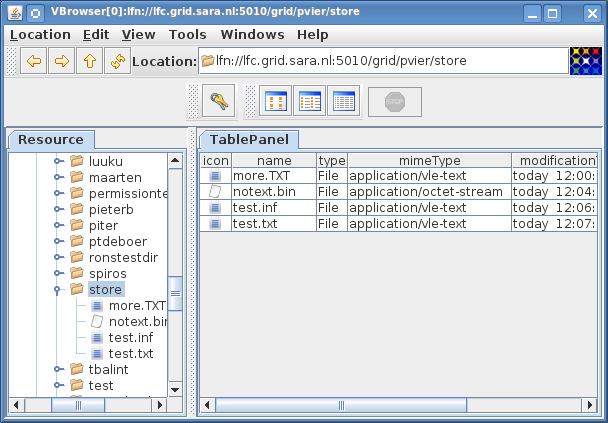
\includegraphics[scale=0.5]{vbrowser_custom_icons}}
\caption{Custom Icons}
\label{fig:custom_icons}
\end{figure}\\
\\
You can also put the icon in your installation by creating it at the following
path:\\
\\
\tab \Path{VLET\_INSTALL/lib/icons/mimetypes/application-vle-text.png}\\

\subsection{Viewer preferences and defaults}

To specify which viewer (vbrowser plugin) is used the user can configure the file
\Path{HOME/.vletrc/viewerconf.prop}.
This file specifies per line the mimetype and the viewerclass which is started
as default viewer when the user opens or clicks (on) a resource.
The syntax is as follows:\\
\\
\tab \Code{mimetype/mimesubtype=viewerclass}\\
\\
For example to specify a new viewer for the ``application/vle-text'' mimetype,
add a line as follows:\\

\begin{boxedlisting}
\begin{verbatim}
##
# File    : viewerconf.prop 
# Location: $HOME/.vletrc/viewerconf.prop
#---
# Mimetype/viewer class mapping file 
# <MIMETYPE>=<VIEWERCLASS> 

# viewerclass mapping for the application/vle-text mimetype:
application/vle-text=nl.uva.vlet.gui.viewers.HexViewer

# end viewerconf.prop file 
\end{verbatim}
\end{boxedlisting}\\
\\
Now, instead of the default textviewer, the actual bytes will be shown in the 
HexViewer utility.\\
Other default vbrowser internal viewer classes are:
\begin{verbatim}
	nl.uva.vlet.gui.viewers.TextViewer
	nl.uva.vlet.gui.viewers.HexViewer 
	nl.uva.vlet.gui.viewers.VHTMLViewer
	nl.uva.vlet.gui.viewers.ImageViewer
\end{verbatim}

For information about how to create custom plugins, see the VLET Developers 
Guide (ref:[]).


  
\newpage

%% Chapter 3 
%
% VBrowser
%

\appendix
\chapter{Appendices}
\label{chap:appendices}

\section{VRL specification} 

This appendix specifies the syntax used for VRLs (Virtual Resource Locators)
which follows the specification of URIs (Universal Resource Indicators) as
specified in \cite{bernerslee2005uri}.\\
In short a VRL is an URI, but not all URIs are VRLs.\\
\par
VRLs can be seen as Virtual URLs which may have extra schemes which do not map
to an actual network protocol but to an 'Virtual' Protocol or 'VRS' Driver
protocol (VDriver). An example is 'rfts' which is not an actual network protocol but is
implemented as Grid Service protocol to an Reliable File Transfer Service. The
actual network protocol used is SOAP messages over https connections as
specified in the WSRF specifications. This is hidden for the user. \\

\subsection{Syntax} 

\hspace*{10mm}\begin{minipage}{170mm}
\begin{verbatim}
 VRL                ::= SCHEME + ':' + SCHEMESPECIFICPART

 SCHEMESPECIFICPART ::=   [ '//' + AUTHORITY ]  
                        + [ '/' + PATH ] 
                        + [ '?' + QUERY ] 
                        + [ '#' + FRAGMENT ]

 AUTHORITY          ::=  [ USERINFO + '@' ] + [ HOSTNAME + [ ':' + PORT ] ]  

 SCHEME             ::= 'file', 'gftp', 'sftp', 'http', 'lfn', 'srm', ..

 USERINFO           ::= USERNAME + [ '.' + DOMAINNAME ] + [ ':' + PASSWORD ]

 USERNAME           ::= UNRESERVED <see rfc3986> 

 DOMAINNAME         ::= UNRESERVED <see rfc3986>

 HOSTNAME           ::= UNRESERVED <see rfc3986> 

 PASSWORD           ::= UNRESERVED <see rfc3986>

 QUERY              ::= UNRESERVED <see rfc3986>
	
 FRAGMENT           ::= UNRESERVED <see rfc3986>

 UNRESERVED         ::= [ ALPHA | NUM |  '-' | '.' | '_' | '~' ] * 

\end{verbatim}
\end{minipage}\\
\\
\Note{Notes:}
\begin{itemize}
%   \item SRB URIs have a \Variable{DOMAINNAME} in the \Variable{USERNAME} part. 
%         VRLs will take the last dot separated string as domain name. 
%         For example in 'john.doe.vle', the 'vle' part is the domain name 
%         and 'john.doe' the username. 
  \item It is not recommended putting plain text passwords in URIs as this 
        is a security hazard. 
  \item The AUTHORITY part start with two slashes '//' but is optional. When
        the scheme specific part starts with only one slash it has no authority
        part.
\end{itemize}

\subsection{Examples of URIs}

This section explains how URIs (VRLs) are used in VLET/VBrowser .\\  
Below an example of a full URI.

\hspace*{10mm}\begin{minipage}{170mm}
\begin{verbatim}
     foo://john_doe@example.com:8042/over/there?name=ferret#nose
     \_/   \_______________________/\_________/ \_________/ \__/
      |              |                |            |         |
    scheme       authority           path        query    fragment
\end{verbatim}
 \end{minipage}\\

After the first colon (':') the \emph{scheme specific} part starts. 
This part can contain an authority part which always starts with two slashes
('//').\\
For example:\\
\\
  \tab \path{sftp://skoulouz@ui.grid.sara.nl:22/data/home/skoulouz}\\
\\
The \emph{authority} part can be omitted if for the scheme no authority is
needed. In that case the scheme specific part may NOT start with two slashes,
but only one in for example in the following URI:\\
\\
   \tab (1) \path{file:/home/dexter/e-laboratory}\\
\\
This is equivalent with an empty \emph{authority} URI as follows:\\
\\
   \tab (2) \path{file:///home/dexter/e-laboratory}\\ 
\\ 
The above URI (2) will be normalized to (1) to indicate an empty authority
part and remove superfluous slashes.\\
\\
\subsection{URI Attributes}

An URI can have URI attributes specified in the \emph{query} part. Some scheme
implementations support URI attributes to specify extra options or parameters
to the underlying implementation. \\
The syntax is as follows:\\ 
\\
\hspace*{10mm}\begin{minipage}{170mm}
\begin{verbatim}
 QUERY         ::= [ ParameterList ]  

 ParameterList ::=  Parameter + [ '&' + ParameterList ]

 Parameter     ::=   Name + '=' +  Value

\end{verbatim}
 \end{minipage}\\
\\
\\
Example of two URI Attributes in an LFC URI:\\
\\
\hspace*{10mm}\begin{minipage}{170mm}
\begin{verbatim}
 lfn://lfc.grid.sara.nl/grid/vlemed/stuff\
      ?lfc.listPreferredSEs=srm.grid.sara.nl\
      &lfc.replicaSelectionMode=Preferred
\end{verbatim}
\end{minipage}\\
\\
% \\
% Or specifying properties for LFC resources: \\
% \\
% \hspace*{10mm}\begin{minipage}{170mm}
% \begin{verbatim}
%  lfn://lfc.grid.sara.nl/grid/vlemed/stuff\
%      ?lfc.listPreferredSEs=srm.grid.sara.nl
% \end{verbatim}
% \end{minipage}\\
% \\
(Remove the backslash '\bsl' when concatenating the URI parts). \\
You can use this feature when invoking the \path{uricopy.sh} script or accessing
the VRS programmatically.
\par
Most properties which can be specified as Resource Properties using the
VBrowser can be specified here although not all combinations have been tested
and some are implementation specific. Check the documentation of the specific
protocol implementation to see which property is supported. 
\par
Don't forget to prepend the property with the name of the scheme, like in
\path{'lfc.listPreferredSEs'} to indicate the \path{lfc} property
\path{listPreferredSEs}. That is when lfc is replicating a file, it will use the storage elements indicated after the \path{'lfc.listPreferredSEs='} which for the example above would be srm.grid.sara.nl

%%%
%%%
%%%

\newpage
\section{Overview of configuration files and directories}

The next sections show an overview of the distribution and user
configuration files. See chapter \ref{chap:customization} for the
customization of these files.

\subsection{Installation files and settings}

 Selection of configuration files and directories in the VLET distribution
 replace \path{VLET_INSTALL} with the location of the distribution):\\
 \\
 \begin{tabular}{ l l }
   \path{VLET_INSTALL/etc} & Directory where all distribution settings are.\\
   \path{VLET_INSTALL/etc/vletrc.prop} & Installation properties and (default)
        settings.\\
   \path{VLET_INSTALL/etc/certificates} & Extra trusted CA root certificates.\\
   \path{VLET_INSTALL/etc/vomsdir/voms.xml} & VO Server configuration.\\
   \path{VLET_INSTALL/lib/plugins} & Custom VDriver plugins and VBrowser
        Viewers.\\
 \end{tabular}
 

\subsection{Default installation configuration file vletrc.prop} 

The default settings for SRB and for LFC can be found in
\path{VLET_INSTALL/etc/vletrc.prop}.\\
These are the default properties used when creating a new resource or contact
remote resources.\\
Most of these properties can also be specified during startup or as extra URI
attribute in the URI (VRL).\\
\\
% \subsubsection{Default SRB settings} 
% 
% Below an example of SRB properties found in
% \path{VLET_INSTALL/etc/vletrc.prop}. \\
% \\
% \begin{boxedlisting}
% \begin{verbatim}
% 
% ###
% # Default SRB host at SARA :
% #
% 
% srb.hostname=srb.grid.sara.nl
% srb.path=/VLENL/home
% srb.port=50000
% srb.mdasCollectionHome=/VLENL/home
% srb.mdasDomainHome=vlenl
% srb.mdasDomainName=vlenl
% srb.defaultResource=vleGridStore
% #srb.username=
% srb.mcatZone=VLENL
% # set to true when behind a firewall (Default)
% # if incoming connection are allowed set to 'false'
% srb.passiveMode=true
% #this string MUST match the Enum Value for 'GSI_AUTH'
% srb.AUTH_SCHEME=GSI_AUTH
% 
% \end{verbatim} 
% \end{boxedlisting}

\subsubsection{Default LFC settings} 

The default settings for LFC which can be found in
\path{VLET_INSTALL/etc/vletrc.prop}. \\
\\
\begin{boxedlisting}
\begin{verbatim}

## Default LFC Server settings: 
## 
# Default LFC hostname: Specify empty field for the user to fill in. 
#lfc.hostname=lfc.grid.sara.nl
lfc.hostname=<LFCHOST>
# Default port: 
lfc.port=5010
## Example of preconfigured Storage Elements:
#lfc.listPreferredSEs=srm.grid.sara.nl,tbn18.nikhef.nl
lfc.replicaNrOfTries=5
## Replica selection mode (reading). 
## One of: Preferred, PrefferedRandom, AllSequential, AllRandom
#lfc.replicaSelectionMode=PreferredRandom
## Replica creation mode (writing) 
## One of:  Preferred, PrefferedRandom, DefaultVO, DefaultVORandom
#lfc.replicaCreationMode=Preferred
## replica naming policy. One of: Similar,Random 
#lfc.replicaNamePolicy=Similar

\end{verbatim} 
\end{boxedlisting}

\subsection{User configuration files}
 
 All the user configurations are stored in the users home directory
 under \path{.vletrc}.\\
 An overview of current used directories and files are (replace HOME with the
 user's home directory):
 \\
 \\
 \begin{tabular}{ l l }
   \path{HOME/.vletrc/} & Directory where user configuration files are stored.\\
   \path{HOME/.vletrc/vletrc.prop} & User property settings.\\
   \path{HOME/.vletrc/cacerts} & User trusted certificates.\\
   \path{HOME/.vletrc/certificates/} & Directory for extra user trusted (CA) certificates.\\ 
   \path{HOME/.vletrc/guisettings.prop} & User GUI (VBrowser) settings.\\
   \path{HOME/.vletrc/mime.types} & User configured mime types.\\
   \path{HOME/.vletrc/viewerconf.prop} & User mime type to Viewer mapping.\\
   \path{HOME/.vletrc/myvle/} & User's 'My Grid' environment.\\
   \path{HOME/.vletrc/icons/} & User customized icons.\\
   \path{HOME/.vletrc/icons/mimetypes/} & User mimetype icons.\\
   \path{HOME/.vletrc/icons/mimetypes/text-plain.png} & Example User
      customized icon for mime type 'text/plain'.\\
   \path{HOME/.vletrc/plugins/} & User Installed plugins.\\

 \end{tabular}
\\

\subsection{Example user customized mime.types file}

The file \path{HOME/.vletrc/mime.types} contains 
user customized mime types. \\
See \ref{chap:customization}  how to customize this file.\\ 
\\
  \begin{boxedlisting}[170]
\begin{verbatim}
###
# File    : mime.types
# Location: $HOME/.vletrc/mime.types
# ---
# Default mime types:  <MIMETYPE>  <EXTENSION1> <EXTENSION2> ...
#

# example vle text mime type: 
application/vle-text          vletxt txt TXT

# example vlemed mime types:  
application/vlemed-fslview    nii nii.gz NII NII.GZ
application/jglite-jobids     vljids
application/taverna-scufl     scufl
application/feat-fsf          fsf FSF 

#end default mime types file 
\end{verbatim}
\end{boxedlisting}
 
\subsection{Example user customized viewerconf.prop file}

The file \path{HOME/.vletrc/viewerconf.prop} contains 
user customized mime type to (VBrowser) Viewer mappings.\\ 
See \ref{chap:customization}  how to customize this file. \\
\\
\begin{boxedlisting}
\begin{verbatim}
##
# File    : viewerconf.prop 
# Location: $HOME/.vletrc/viewerconf.prop
#---
# Mimetype/viewer class mapping file. NO spaces between '=' !.  
# <MIMETYPE>=<VIEWERCLASS> 

# Example viewer mapping for the application/vle-text mimetype:
application/vle-text=nl.uva.vlet.gui.viewers.TextViewer

# Example vlemed mimetype and to viewer mapping: 
application/vlemed-fslview=nl.amc.vlet.feat.fslview.gui.ViewerFSL
application/taverna-scufl=nl.uva.vlet.moteur.plugin.gui
application/jglite-jobids=nl.uva.vlet.monitoring.gui.ViewerGliteJobMonitoring
application/feat-fsf=nl.amc.vlet.feat.client.main.gui.ViewerFeatParameterSweep

# end viewerconf.prop file 
\end{verbatim}
\end{boxedlisting}\\
\\

 
  
\newpage

%% Bibliography
\bibliography{biblio}
\bibliographystyle{plain}

\end{document} 

